\documentclass[11pt, a4paper]{article}
\usepackage[utf8]{inputenc}
\usepackage{amsmath,setspace,geometry}
\usepackage{amsthm}
\usepackage{amsfonts}
\usepackage{mathtools}
\mathtoolsset{showonlyrefs}
\usepackage[shortlabels]{enumitem}
\usepackage{rotating}
\usepackage{pdflscape}
\usepackage{graphicx}
\usepackage{bbm}
\usepackage[dvipsnames]{xcolor}
\usepackage[colorlinks=true, linkcolor= RawSienna, citecolor = RawSienna, filecolor = RawSienna, urlcolor = RawSienna, hypertexnames = true, backref = page]{hyperref}
\usepackage[]{natbib} 
\bibpunct[:]{(}{)}{,}{a}{}{,}
\geometry{left = 1.0in,right = 1.0in,top = 1.0in,bottom = 1.0in}
\usepackage[english]{babel}
\usepackage{float}
\usepackage{caption}
\usepackage{subcaption}
\usepackage{tikz}
\usepackage{booktabs}
\usepackage{pdfpages}
\usepackage{framed} % For boxed environment
\usepackage{threeparttable}
\usepackage{lscape}
\usepackage{bm}
\usepackage{comment}
\setstretch{1.3}
%\usepackage[tablesfirst,nolists]{endfloat}

\usepackage[T1]{fontenc}
\usepackage{mlmodern}  % 太いComputer Modern
% MLmodernのバグを修正: cf. https://tex.stackexchange.com/questions/646333/size-of-integral-symbol-in-section-header-with-mlmodern
\DeclareFontFamily{OMX}{mlmex}{}
\DeclareFontShape{OMX}{mlmex}{m}{n}{<->mlmex10}{} 
\usepackage{tgtermes} % 数式以外の欧文をTXフォントで上書き

\newtheorem{theorem}{Theorem}
\newtheorem{assumption}{Assumption}
\newtheorem{lemma}{Lemma}
\newtheorem{definition}{Definition}
\newtheorem{proposition}{Proposition}
\newtheorem{claim}{Claim}
\newtheorem{corollary}{Corollary}
\newtheorem{example}{Example}
\DeclareMathOperator{\rank}{rank}

\theoremstyle{remark}
\newtheorem{remark}{Remark}


\title{A Note on Identifying Conduct Parameters with Separable Demand of \cite{lau1982identifying}}
\author{Yuri Matsumura\thanks{Department of Economics, Rice University, \href{mailto:}{yuri.matsumura23@gmail.com}} \and Suguru Otani \thanks{Market Design Center, Department of Economics, University of Tokyo, \href{mailto:}{suguru.otani@e.u-tokyo.ac.jp}
\\Declarations of interest: none %this is for Economics Letters
}}

\begin{document}

\maketitle
\begin{abstract}
    We provide a counterexample to the conduct parameter identification result established in the foundational work of \citet{lau1982identifying}, which generalizes the identification theorem of \citet{bresnahan1982oligopoly} by relaxing the linearity assumptions. We identify a separable demand function that permits identification and validate this case theoretically and through numerical simulations.
\end{abstract}

\noindent\textbf{Keywords:} Conduct parameters, Homogenous Goods Market, Monte Carlo simulation
\vspace{0in}
\newline
\noindent\textbf{JEL Codes:} C5, C13, L1

\bigskip

\section{Introduction}

Measuring market power is a fundamental task in Industrial Organization. 
The conduct parameter approach provides a robust framework for evaluating market power, and a substantial body of empirical research has focused on identifying this parameter. 
\cite{bresnahan1982oligopoly} and \citet{lau1982identifying} provide fundamental results on identifying the conduct parameter.
First, \citet{bresnahan1982oligopoly} establishes key conditions for identifying the conduct parameter in a homogeneous product market, assuming a linear demand function and linear marginal costs. 
Second, \citet{lau1982identifying} extends this identification framework by relaxing the linearity assumptions.

In this note, we provide a counterexample to the identification result in \citet{lau1982identifying}. 
The paper argues that the separability of the demand function, a concept introduced by \citet{goldmanNote1964}, is critical for identification. 
Specifically, the conduct parameter and the marginal cost function can be identified when the demand function is non-separable or follows a particular separable form.
In contrast, we identify a separable demand function that does not conform to the particular form yet still allows identification. 

\section{Model}
Consider a homogeneous product market.
The aggregate inverse demand and aggregate marginal cost function are given as
\begin{align}
    P = f(Q, X^{d}), \label{eq:demand}
    \\
    MC = g(Q, X^{s}),\label{eq:marginal_cost}
\end{align}
where $Q$ is the aggregate quantity, $X^{d}$ and $X^{s}$ are the vector of exogenous variables.
Assume that $X^{d}$ and $X^{s}$ are exclusive, that is, there is no common variable in $X^{d}$ and $X^{s}$.
In this sense, $X^{d}$ works as demand shifter and $X^{s}$ works as cost shifter. 
Then, we obtain the supply equation:
\begin{align}
     P + \theta\frac{\partial P(Q)}{\partial Q}Q = MC,\label{eq:supply_equation}
\end{align}
where $\theta\in[0,1]$, which is the conduct parameter. 
The equation nests perfect competition ($\theta=0$) and perfect collusion ($\theta=1$) (See \cite{bresnahan1982oligopoly}). 

\citet{lau1982identifying} considers the identification of the conduct parameter and the marginal cost function. 
Instead of directly proving identification, \citet{lau1982identifying} takes an indirect approach by specifying the conditions under which the model is not identified. 
The definition of non-identification in this model is as follows:
\begin{definition}\label{def:non_identification}
    Non-identification implies for any $X^{d}$ and $X^{s}$,
    \begin{align}
    f(Q, X^{d}) + \theta \frac{\partial f}{\partial Q}(Q, X^{d})Q &= g(Q, X^{s}),  \label{eq:foc_alpha}\\
    f(Q, X^{d}) + \theta' \frac{\partial f}{\partial Q}(Q, X^{d})Q &= g'(Q, X^{s}),\label{eq:foc_beta}
    \end{align}
    where $\theta \neq \theta'$, $g \ne g'$,\footnote{This condition is not stated in \citet{lau1982identifying}, but assuming $g = g'$ makes the identification simple.} and the reduced form functions $Q = h(X^{d}, X^{s})$ and $Q = h'(X^{d}, X^{s})$ defined by \eqref{eq:foc_alpha} and \eqref{eq:foc_beta} respectively are identical.
\end{definition}
In other words, non-identification asks the following question: given an identified demand function $f$, is it possible to find two distinct pairs of conduct parameter and marginal cost, $\Lambda = (\theta, g)$ and $\Lambda' = (\theta', g')$, that lead to observable equivalent equilibrium?

\citet{lau1982identifying} presents the condition on the demand function under which the conduct parameter cannot be identified:
\begin{theorem}\label{theorem_lau}
    Under the assumption that the industry inverse demand and cost functions are twice continuously differentiable, the index of competitiveness $\theta$ cannot be identified from data on industry price and output and other exogenous variables alone if and only if the industry inverse demand function is separable in $X^{d}$, that is,
    \begin{align}
        P = f(Q, r(X^{d})), \label{eq:demand_separable}
    \end{align}
    but not take the form, 
    \begin{align}
        P = Q^{-1/\theta}r(X^{d}) + s(Q). \label{eq:identification_separable}
    \end{align}
\end{theorem}
The theorem implies that the conduct parameter is identified when the demand function is not separable, except \eqref{eq:identification_separable}.


While the 





\subsection{Relation to the recent literature on distinguishing firm conduct}

The sufficiency of separability implies that if the conduct parameter and marginal cost are simultaneously identified, the demand function is non-separable or satisfies the specific separable function form.
However, the recent literature uses a broader variation in markets for the identification of conduct beyond demand shifters and rotators.
For example, in the differentiated product environment, \citet{berry2014identification} demonstrate that the change in marginal cost or the market size is useful, and hence demand rotation instruments are not necessary to identify conduct.

Of course, homogeneous product settings are more restricted than differentiated product settings.
Even so, Lau's proof of sufficiency does not show that unless a separable demand satisfies  \eqref{eq:identification_separable}, there always exist two distinct pairs of conduct parameter and marginal cost.
Therefore, there could be a separable function except \eqref{eq:identification_separable} that can achieve identification based on other variations in markets.

\section{Conclusion}

%We present a counterexample to \citet{lau1982identifying}'s identification result, showing that a separable demand function outside his specified form can still achieve identification of both the conduct parameter and the marginal cost. This finding, supported by theoretical analysis and numerical simulations, challenges existing assumptions for identifying the conduct parameter beyond the linear specification of demand and marginal cost functions.

\paragraph{Acknowledgments}
%We thank Jeremy Fox and an anonymous referee for their invaluable comments and Kaede Hanazawa for his excellent research assistance.
This work was supported by JST ERATO Grant Number JPMJER2301, Japan.  

\bibliographystyle{aer}
\bibliography{conduct_parameter.bib}

\iffalse
\appendix
\section{Appendix}


\subsection{A counterexample}

Now, we show that the conduct parameter is identified when the inverse demand function is separable. 
Consider the following inverse demand function and marginal cost function:
\begin{align}
    P & = \exp(\varepsilon_{d}) Q^{\alpha_0} (X_{1}^{d})^{\alpha_1}(X_{2}^{d})^{\alpha_2}\label{eq:counter_demand}\\
    MC & = \exp(\varepsilon_{s})Q^{\beta_0} (X_{1}^{s})^{\beta_1} (X_{2}^{s})^{\beta_2},\label{eq:counter_mc}
\end{align}
where $\varepsilon_{d}$ and $\varepsilon_{s}$ satisfy the mean independence condition $E[\varepsilon_{d}|X^{d}, X^{s}] = E[\varepsilon_{s}|X^{d}, X^{s}] =0$. 
Assume that $\alpha_0 \ne -1/\theta$, so as not to satisfy the specific functional form \eqref{eq:identification_separable}.

The inverse demand \eqref{eq:counter_demand} is separable because
\begin{align}
    \frac{\partial }{\partial Q} \left(\frac{\partial P/\partial X_{1}^{d}}{\partial P/\partial X_{2}^{d}} \right) = \frac{\partial }{\partial Q} \left(\frac{\alpha_{1}\exp(\varepsilon_{d}) Q^{\alpha_0} (X_{1}^{d})^{\alpha_1-1}(X_{2}^{d})^{\alpha_2}}{\alpha_2\exp(\varepsilon_{d}) Q^{\alpha_0} (X_{1}^{d})^{\alpha_1}(X_{2}^{d})^{\alpha_2-1}} \right) =  \frac{\partial }{\partial Q}\left(\frac{\alpha_1}{\alpha_2} \frac{X_{2}^{d}}{X_{1}^{d}} \right)=0.
\end{align}

By taking the logarithm of the inverse demand \eqref{eq:counter_demand}, we have a log-linear demand equation such that 
\begin{align}
    \log P = \alpha_0 \log Q + \alpha_1 \log X_{1}^{d}  + \alpha_2 \log X_{2}^{d} + \varepsilon_{d}.\label{eq:counter_demand_equation}
\end{align}
The demand parameters can be identified when $X^s$ is a vector of exclusive demand instruments.
Thus, we can assume that $\alpha_0, \alpha_1$, and $\alpha_2$ are known.  

The left-hand side of the first-order condition \eqref{eq:supply_equation} can be written as
\begin{align}
    P + \theta\frac{\partial P(Q)}{\partial Q}Q & =  P + \theta [\alpha_0 \exp(\varepsilon_{d})Q^{\alpha_0-1}(X_{1}^{d})^{\alpha_1}(X_{2}^{d})^{\alpha_2}] Q\\
    & = P + \theta \alpha_0 P\\
    &= (1 + \theta\alpha_0) P.
\end{align}
Substituting this and the marginal cost function \eqref{eq:counter_mc} into the supply equation \eqref{eq:supply_equation} and taking a logarithm, we obtain the log-linear supply equation,
\begin{align}
    \log P = - \log(1 + \theta\alpha_0) + \beta_0 \log Q + \beta_1 \log X_{1}^{s}+\beta_2 \log X_{2}^{s} + \varepsilon_{s}.\label{eq:counter_supply_equation}
\end{align}
Let $\gamma = - \log(1 + \theta\alpha_0)$. When $X^d$ and $X^s$ contain non-overlapping variables, $X^d$ serves as a vector of instrumental variables for the supply equation. 
Applying the identification argument for instrumental variable regression, the parameters $\gamma$, $\beta_0$, and $\beta_1$ are identified. 
Consequently, the parameter $\theta$ is also identified as $\theta = (\exp(-\gamma) - 1)/\alpha_0$, which contradicts Theorem \ref{theorem_lau}. 
%Note that we do not need to introduce Bresnahan demand rotation instruments, discussed in \cite{matsumura2023resolving}.


A critical remark is that the demand function exhibits constant elasticity, and \citet{lau1982identifying} states in his conclusion that it is impossible to identify the conduct parameter under the demand function unless $\alpha_0 = -1/\theta$. 
When this happens in the counterexample, the constant term in \eqref{eq:counter_supply_equation} becomes $\gamma = -\infty$, so the supply equation can adequately defined.
Therefore, the counterexample achieves the identification under the condition where \citet{lau1982identifying} states it is impossible and cannot achieve the identification under the condition where he states it is possible. Numerical validation is shown in Appendix \ref{sec:simulation}.


\subsection{Omitted Proof for Proposition 1}\label{sec:omit_proof}

Note that from \eqref{eq:counter_demand_equation} and \eqref{eq:counter_supply_equation}, the equilibrium quantity is given as
\begin{align}
    \log Q &= \frac{ \log (1 + \theta \alpha_0 )}{\beta_0 - \alpha_0} + \frac{\alpha_1 \log X_{1}^{d} + \alpha_2 \log X_{2}^{d} - \beta_1 \log X_{1}^{s} - \beta_2 \log X_{2}^{s} + \varepsilon^{d} - \varepsilon^{c}}{\beta_0 - \alpha_0 }.\label{eq:quantity_loglinear}
\end{align}
Let $\Lambda = (\theta, \beta_0, \beta_1, \beta_2)$ and  $\Lambda' = (\theta', \beta_0', \beta_1', \beta_2')$ be distinct sets of parameters.
Assume at least $\theta\ne \theta'$ holds.
Define the reduced from function for the equilibrium quantity as $Q = h(X^d, X^s; \Lambda)$.
Because taking logarithm does not change the relationship, two models with $\Lambda$ and $\Lambda'$ are observably equivalent when
\begin{align}
    \log Q = \log h(X^d, X^s; \Lambda) = \log h(X^d, X^s; \Lambda') \quad \text{ for all } X^d, X^s.
\end{align}

Then take a derivative of \eqref{eq:quantity_loglinear} with $X^d_{i}$ and $X^s_{i}$ for $i = 1,2$, we have
\begin{align}
    \frac{\partial \log Q}{\partial X^{d}_i} = \frac{\alpha_i}{\beta_0 - \alpha_0} \frac{1}{X_{i}^d} =  \frac{\alpha_i}{\beta_0' - \alpha_0} \frac{1}{X_{i}^d} ,\label{eq:non_identifiy_derivative_d}\\
    \frac{\partial \log Q}{\partial X^{s}_i} = \frac{\beta_i}{\beta_0 - \alpha_0} \frac{1}{X_{i}^s} =  \frac{\beta_i'}{\beta_0' - \alpha_0} \frac{1}{X_{i}^s} .\label{eq:non_identifiy_derivative_s}
\end{align}
\eqref{eq:non_identifiy_derivative_d} implies $\beta_0 = \beta_0'$.
If $\beta_0 \ne \beta_0'$ under $\Lambda$ and $\Lambda'$, this immediately leads to a contradiction.
If $\beta_0 = \beta_0'$, \eqref{eq:non_identifiy_derivative_s} implies $\beta_i =\beta_i'$ for $i = 1,2$, which concludes the marginal cost parameters are all the same under $\Lambda$ and $\Lambda'$.
Again, if one of the marginal cost parameters is different under $\Lambda$ and $\Lambda'$, it leads to a contradiction.
Suppose that the marginal cost is the same under $\Lambda$ and $\Lambda'$.
However, it is obvious from \eqref{eq:quantity_loglinear} that $\log h(X^d, X^s; \Lambda) = \log h(X^d, X^s; \Lambda')$ cannot hold because the first term is different while the second term is the same under $\Lambda$ and $\Lambda'$.
Therefore, the model in the counterexample cannot have distinct sets of parameters that lead to observable equivalent equilibrium.


\begin{remark}

The total revenue is
\begin{align}
    TR = PQ = \exp(\varepsilon_{d}) Q^{\alpha_0+1} (X_{1}^{d})^{\alpha_1}(X_{2}^{d})^{\alpha_2},
\end{align}
and hence the marginal revenue is
\begin{align}
    MR = (\alpha_0+1)\exp(\varepsilon_{d}) Q^{\alpha_0}  (X_{1}^{d})^{\alpha_1}(X_{2}^{d})^{\alpha_2}.
\end{align}
Take the logarithm of the marginal revenue, we have
\begin{align}
    \log MR& = \log (1 + \alpha_0) + \alpha_0 \log Q + \alpha_1 \log X_{1}^{d} + \alpha_2 \log X_{2}^{d} + \varepsilon_d.
\end{align}
The marginal revenue function shifts the demand function by $\log (1 + \alpha_0)$.
\end{remark}

\begin{figure}[t]
    \centering
        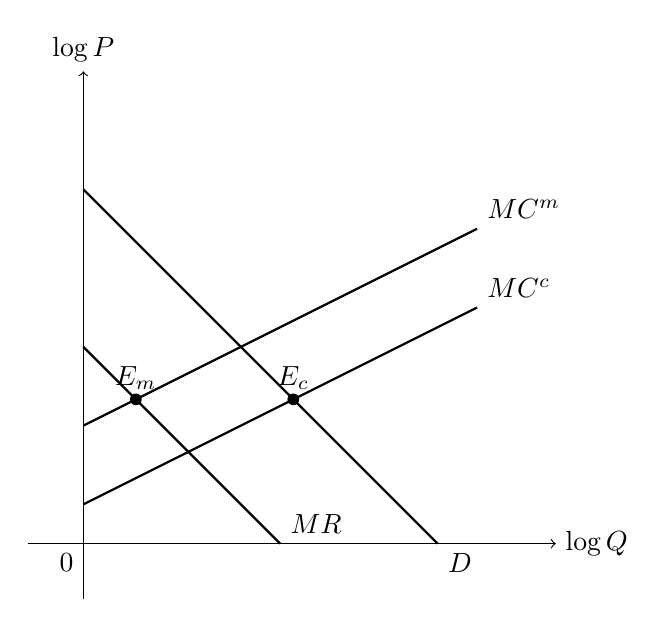
\begin{tikzpicture}
            % Axes
            \draw[->] (-0.7,0) -- (6,0) node[right] {$\log Q$}; % Horizontal axis
            \draw[->] (0,-0.7) -- (0,6) node[above] {$\log P$}; % Vertical axis

            % Marginal Revenue (MR_1) - passes through (0,5), (3,2), and (5,0)
            \draw[thick] (0,4.5) -- (4.5,0) node[below right] {$D$};
            \draw[thick] (0,2.5) -- (2.5,0) node[above right] {$MR$};
            
            % Supply Curve under competition (S^c) - passes through (0,1), (3,4), and (4.5,5.5)
            \draw[thick] (0,1.5) -- (5,4) node[above right] {$MC^m$};
            % Supply Curve under monopoly (S^m) - passes through (0,1), (3,2), and (7.5,3.5)
            \draw[thick] (0,0.5) -- (5,3) node[above right] {$MC^c$};

            % Equilibrium point (E_1) - intersection of D_1 and S^c at (3,4)
            \node[circle, fill, inner sep=1.5pt] (Ec) at (2/3,11/6) {};
            \node[above] at (Ec) {$E_m$};

            \node[circle, fill, inner sep=1.5pt] (Em) at (8/3,11/6) {};
            \node[above] at (Em) {$E_c$};
            % Additional labels
            \node[below left] at (0,0) {0};
            %\node[below] at (2/3, 0) {$Q_m$};
            %\node[below] at (8/3, 0) {$Q_c$};

            %\draw[dashed] (8/3,0) -- (8/3,11/6);
            %\draw[dashed] (2/3,0) -- (2/3,11/6);
        \end{tikzpicture}
        \caption{}
    \caption{Identification of the conduct under the log-linear model}
    \label{fig:simpe_identification}
\end{figure}










\subsection{Simulation}\label{sec:simulation}
We validate our counterexample numerically via Monte Carlo simulation as in \cite{matsumura2023resolving}.
We set true parameters and distributions as shown in Table \ref{tb:parameter_setting}.
Note that under the parameter setting, the inverse demand function does not satisfy \eqref{eq:demand_separable}, which is a specific separable function leading to the identification.
For the simulation, we generate 1,000 data sets. 
The demand and supply equations are estimated separately using two-stage least squares (2SLS) estimation. The instrumental variables for the demand estimation are $(Z_{1}^{s}, Z_{2}^{s})$, and for the supply estimation, the instrumental variables are $(X_{1}^{d}, X_{2}^{d})$. 
As reported in Table \ref{tb:counterexample_for_Lau1982_sigma_0.001_bias_rmse}, biases and RMSEs decrease sharply as the sample size increases. 
This confirms our finding that our counterexample successfully achieves conduct parameter identification.

\begin{table}[!htbp]
    \caption{True parameters and distributions}
    \label{tb:parameter_setting}
    \begin{center}
    \subfloat[Parameters]{
    \begin{tabular}{cr}
            \hline
            & linear  \\
            $\alpha_0$ & $-1.0$  \\
            $\alpha_1$ & $1.0$  \\
            $\alpha_2$ & $1.0$ \\
            $\beta_0$ & $1.0$ \\
            $\beta_1$ & $1.0$  \\
            $\beta_2$ & $1.0$ \\
            $\theta$ & $0.5$ \\
            \hline
        \end{tabular}
    }
    \subfloat[Distributions]{
    \begin{tabular}{crr}
            \hline
            & linear\\
            Demand shifter&  \\
            $X_{1}^{d}$ & $U(1,3)$  \\
            $X_{2}^{d}$ & $U(1,3)$  \\
            Cost shifter&    \\
            $X_{1}^{s}$ & $U(1,3)$   \\
            $X_{2}^{s}$ & $U(1,3)$  \\
            $Z_{1}^{s}$ & $\log X_{1}^{s} +N(0,1)$   \\
            $Z_{2}^{s}$ & $\log X_{2}^{s} +N(0,1)$   \\
            Error&  &  \\
            $\varepsilon^{d}$ & $N(0,\sigma)$  \\
            $\varepsilon^{s}$ & $N(0,\sigma)$ \\
            \hline
        \end{tabular}
    }
    \end{center}
    \footnotesize
    Note: $\sigma=\{0.001, 0.5, 1.0\}$. $N:$ Normal distribution. $U:$ Uniform distribution. The replication code is available on the author's github. Note that the value of $\alpha_0$ and $\theta$ does not satisfy the functional form in \eqref{eq:identification_separable}
\end{table}

\begin{table}[!htbp]
  \begin{center}
      \caption{Results of the separable demand model}
      \label{tb:counterexample_for_Lau1982_sigma_0.001_bias_rmse} 
      \subfloat[$\sigma=0.001$]{
\begin{tabular}[t]{llrrrrrrr}
\toprule
  & Bias & RMSE & Bias & RMSE & Bias & RMSE & Bias & RMSE\\
\midrule
$\alpha_{0}$ & 0.000 & 0.005 & 0.000 & 0.003 & 0.000 & 0.002 & 0.000 & 0.001\\
$\alpha_{1}$ & 0.000 & 0.001 & 0.000 & 0.001 & 0.000 & 0.001 & 0.000 & 0.000\\
$\alpha_{2}$ & 0.000 & 0.001 & 0.000 & 0.001 & 0.000 & 0.001 & 0.000 & 0.000\\
$\beta_{0}$ & 0.000 & 0.001 & 0.000 & 0.001 & 0.000 & 0.001 & 0.000 & 0.000\\
$\beta_{1}$ & 0.000 & 0.001 & 0.000 & 0.000 & 0.000 & 0.000 & 0.000 & 0.000\\
$\beta_{2}$ & 0.000 & 0.001 & 0.000 & 0.000 & 0.000 & 0.000 & 0.000 & 0.000\\
$\theta$ & 0.000 & 0.001 & 0.000 & 0.001 & 0.000 & 0.000 & 0.000 & 0.000\\
Sample size ($T$) &  & 50 &  & 100 &  & 200 &  & 1000\\
\bottomrule
\end{tabular}
}\\
      \subfloat[$\sigma=0.5$]{
\begin{tabular}[t]{llrrrrrrr}
\toprule
  & Bias & RMSE & Bias & RMSE & Bias & RMSE & Bias & RMSE\\
\midrule
$\alpha_{0}$ & -0.902 & 1.966 & -0.690 & 1.559 & -0.362 & 1.182 & -0.046 & 0.536\\
$\alpha_{1}$ & -0.207 & 0.488 & -0.167 & 0.412 & -0.088 & 0.304 & -0.011 & 0.138\\
$\alpha_{2}$ & -0.231 & 0.537 & -0.169 & 0.388 & -0.085 & 0.299 & -0.010 & 0.134\\
$\beta_{0}$ & 0.016 & 0.751 & -0.013 & 0.494 & 0.007 & 0.337 & -0.006 & 0.143\\
$\beta_{1}$ & -0.002 & 0.326 & 0.002 & 0.208 & 0.005 & 0.146 & 0.003 & 0.063\\
$\beta_{2}$ & -0.008 & 0.309 & 0.013 & 0.213 & -0.001 & 0.141 & 0.004 & 0.065\\
$\theta$ & 0.316 & 1.996 & 0.214 & 1.125 & 0.092 & 0.288 & 0.019 & 0.095\\
Sample size ($T$) &  & 50 &  & 100 &  & 200 &  & 1000\\
\bottomrule
\end{tabular}
}\\
      \subfloat[$\sigma=1.0$]{
\begin{tabular}[t]{llrrrrrrr}
\toprule
  & Bias & RMSE & Bias & RMSE & Bias & RMSE & Bias & RMSE\\
\midrule
$\alpha_{0}$ & 0.101 & 0.464 & 0.046 & 0.318 & 0.023 & 0.223 & 0.009 & 0.096\\
$\alpha_{1}$ & 0.029 & 0.354 & 0.011 & 0.256 & 0.012 & 0.176 & -0.001 & 0.079\\
$\alpha_{2}$ & 0.009 & 0.352 & 0.012 & 0.252 & 0.006 & 0.180 & 0.003 & 0.080\\
$\beta_{0}$ & -0.193 & 0.907 & -0.034 & 0.543 & 0.020 & 0.392 & 0.001 & 0.147\\
$\beta_{1}$ & -0.095 & 0.659 & -0.014 & 0.442 & -0.001 & 0.305 & 0.002 & 0.124\\
$\beta_{2}$ & -0.092 & 0.680 & -0.018 & 0.437 & 0.004 & 0.323 & 0.004 & 0.124\\
$\theta$ & 0.147 & 3.317 & 0.044 & 0.439 & 0.018 & 0.195 & 0.004 & 0.075\\
Sample size ($T$) &  & 50 &  & 100 &  & 200 &  & 1000\\
\bottomrule
\end{tabular}
}
  \end{center}
  \footnotesize
  Note: The error terms in the demand and supply equation are drawn from a normal distribution, $N(0,\sigma)$. 
\end{table} 
\fi

\end{document}